\clearpage
\setcounter{page}{1}
\maketitlesupplementary

\section{Implementation details of STAGS}
\label{sec:suppl:method}

This section lists the details of the final run (\texttt{run\_c.py --recipe E --ladder\_stop 5.5 --posefix\_abc}) that \cref{sec:method} omits.
Notation follows \cref{sec:method}.
% code: runs/engine/runC/run_c.py:main; src: runs/engine/pose_abc_adopt_20261113/blind/launch.json

\subsection{Data, extraction and optics}
\label{sec:suppl:method:data}

\paragraph{Inputs.}
The five tilt series carry RELION's tilt-series alignment (AlignTiltSeries), CTFFIND defocus and per-tilt scale factors, motion-corrected frames and tilt exclusion; the initial picks (Picks/Extract) are oriented along the local surface normal with a random in-plane angle.
Particle names and half-set labels are taken from RELION's final selection (Select/job077, \texttt{rlnRandomSubset}).
% src: runs/engine/inputs/provenance.json ("tilt_series_contents", "selection_source", "pose_source", "a2")
The data have 300\,kV, $C_s=2.7$\,mm, amplitude contrast $w=0.1$, tilt-series pixel 1.35\,\AA\ and handedness $-1$.
% src: runs/engine/inputs/tomograms.star (rlnVoltage, rlnSphericalAberration, rlnAmplitudeContrast, rlnTomoTiltSeriesPixelSize, rlnTomoHand)

\paragraph{Extraction.}
All stacks are written by \texttt{relion\_tomo\_subtomo} with \texttt{--max\_dose 50 --min\_frames 1 --float16 --stack2d}; without \texttt{--no\_ctf} each crop is multiplied by its CTF, and STAGS treats such crops as multiplied by CTF and exposure filter (transfer $T=(cd)^2$).
Crops are 216\,px at bin 2 (2.7\,\AA/px, box 256) for the seed and the ladder down to 6.5\,\AA; 384\,px at bin 1 (box 512) for 5.5\,\AA; 384\,px at bin 1 without CTF multiplication for the optics scan; and 192\,px at bin 1 (box 512) for map fits, P1 and P2, re-extracted after every optics scan.
Each level uses only the Fourier coefficients with $|\bm{\kappa}|\le1/d$.
% code: stags/engine.py:extract, HalfData.set_grid; scripts/lean_chain.py:main (initial extraction bin 2, box 256, crop 216), ladder_config (reextract bin 1, box 512, crop 384); runs/engine/runC/run_c.py:prep_half (crop 192; no_ctf crop RAW_CROP = 384), cycle_E (re-extraction crop 192)

\paragraph{Geometry and optics conventions.}
The tilt rotation of image $j$ is $T_j=R_z(\psi_j)R_y(\theta_j)R_x(\epsilon_j)$ from RELION's ZRot, YTilt and XTilt, and $\Gamma_{ij}=T_jT_{j_0}^{\top}$ with $j_0$ the particle's first image.
% code: stags/relion5_io.py (Rt = Rz(ZRot) Ry(YTilt) Rx(XTilt)); stags/relion5_stags.py:relion_pose_decomposition
In \cref{eq:ctf}, $\Delta f_{ij}(\varphi)=\bar{f}_j+\tfrac12\Delta_j\cos2(\varphi-\varphi_j)+z_{ij}$ combines mean defocus, astigmatism and the depth $z_{ij}$ of the particle in the tilted specimen (handedness $-1$), and $\lambda$ is the relativistic electron wavelength.
The exposure filter is $d_j(\bm{\kappa})=\exp(-N_j/2N_e)$ with $N_e=0.245|\bm{\kappa}|^{-1.665}+2.81$~\cite{grant2015dose}, evaluated at the midpoint exposure $N_j$ of tilt $j$ (pre-exposure plus half the median exposure per tilt).
% code: stags/relion5_io.py:_ctf_parts, wavelength (depth offset, dose = pre + 0.5 dose_per_tilt); stags/optics.py

\paragraph{Whitening and Hermitian weights.}
The weight $w$ is computed per one-pixel shell $\operatorname{round}(|\bm{\kappa}|Nd_{\mathrm{px}})$ from the half's unsubtracted premultiplied images as $\sum T/\sum|\tilde{y}|^2$, shell 0 excluded; $\eta$ is 2 for interior rfft columns and 1 on the DC and Nyquist columns.
% code: stags/likelihood.py:shell_noise_inverse; stags/train.py:fit_half (herm, shell 0 zeroed); stags/engine_search.py:noise_weights

\subsection{Initialization, densification and masks}
\label{sec:suppl:method:init}

\paragraph{Seed model.}
Each half back-projects 250 of its particles at their pick poses (C6 Wiener reconstruction with constant $0.05\cdot\mathrm{mean}$ of the nonzero denominator, trilinear insertion on a twofold grid, gridding correction) and low-passes the map to 40\,\AA\ with a raised cosine from 1/44 to 1/40\,\AA$^{-1}$.
Centers are sampled with probability proportional to the squared positive density inside a 250\,\AA\ sphere, with uniform $\pm\frac12$-voxel jitter; all Gaussians are isotropic with width $d/3$ (5.33\,\AA\ at 16\,\AA) and equal mass, divided by six for the C6 expansion.
One global amplitude is then fitted in closed form, $a=\sum\eta w\operatorname{Re}(\overline{P}\tilde{y})/\sum\eta wT|P|^2$, on 512 images with $|\bm{\kappa}|\le1/40$\,\AA$^{-1}$.
% code: stags_engine.py:main (backproject band_A 16; lowpass 40); stags/engine.py:lowpass, initial_model, fit_amplitude; stags/train.py:seeds_from_volume; stags/relion5_io.py:reconstruct

\paragraph{K schedule.}
At level $d$, the target number of Gaussians (all copies) is
\begin{equation}
K(d)=\operatorname{round}\!\big(0.7\,V/(d/2)^3\big),
\label{eq:kschedule}
\end{equation}
% code: stags/engine.py:k_target_total; scripts/lean_chain.py (MASK_VOLUME_A3, K_CAP = 50000)
with $V=775{,}995$\,\AA$^3$, the volume of RELION's FSC mask (315,397 voxels of $1.35^3$\,\AA$^3$), capped at 50,000.
The targets are 1,061, 2,515, 4,346, 8,487, 15,824 and 26,119 for 16--5.5\,\AA; the cap never binds.
Realized values are 1,056 (176 per asymmetric unit) at 16\,\AA\ and 25,998\,/\,26,046 at 5.5\,\AA.
% src: scripts/lean_chain.py:45 (MASK_VOLUME_A3 = 775994.93); runs/engine/pose_abc_adopt_20261113/blind/lean/ladder/h{1,2}/summary.json (levels[].K_total)

\paragraph{Densification.}
At every level change after 16\,\AA, densification (i)~prunes Gaussians with mass below 1\% of the median or with the center voxel outside the 250\,\AA\ sphere, (ii)~repeatedly splits the widest Gaussians with largest width $s_{\max}>d/3$, widest first and at most up to the target, into children at $\bm{\mu}\pm0.6\,s_{\max}\mathbf{v}$ along the long axis $\mathbf{v}$, with that width scaled by 0.8, half the mass and the parent's orientation, (iii)~would add Gaussians at positive peaks of the back-projected residual if the target were not yet met, (iv)~prunes again and keeps at most the target number of heaviest Gaussians.
In the final run step (iii) never added a Gaussian, because splitting always reached the target.
% code: stags/engine.py:densify; scripts/lean_chain.py:ladder_config (no_densify_levels ["16"]); src: runs/engine/pose_abc_adopt_20261113/blind/lean/ladder/h{1,2}/summary.json (densify.residual_added = 0)

\paragraph{Cold-fit seeding.}
The cold fit uses $K=48{,}000$ (8,000 per asymmetric unit). It is seeded like the seed model from the half's Wiener back-projection at the 5.5\,\AA\ poses (crop 192), multiplied by the mask $M$ and low-passed to 16\,\AA; the global amplitude is fitted on about 256 images with $|\bm{\kappa}|\le1/20$\,\AA$^{-1}$.
Warm fits start from the previous model without refitting the amplitude.
% code: runs/engine/night_20261110/night.py:fit_cmd (--K 48000 --init voxel); stags/relion5_stags.py (init == "voxel": seeds_from_volume(VA * mask, lowpass_A 16); fit_scale kmax 1/20; init_model: no amplitude refit)

\paragraph{Masks.}
The ladder uses a soft 250\,\AA\ sphere (10\,\AA\ cosine edge) only for seeding and pruning.
After the ladder, each half computes its own C6 Wiener back-projection at the 5.5\,\AA\ poses, band-limited to 12\,\AA, filters it to 15\,\AA, and averages it within a radius of 50\,\AA\ about the symmetry axis to obtain an axial profile, with the median beyond $|z|>110$\,\AA\ subtracted and the maximum scaled to 1.
The upper end of the mask is the first point above the center where the profile drops below 0.2; the lower end is found by descending from the center to the local minimum of the profile and then to the first point where it reaches 0.5.
The radius is chosen such that the hard cylinder contains 315,397 voxels, and a 6\,\AA\ cosine edge is added outward.
Because the edge is added outside, the soft mask above 0.5 contains more voxels than the RELION scalar (373,322\,/\,373,831 for the two halves).
The same mask $M$ is used by all later stages; $V_{\mathrm{out}}=V_A(1-M)$ is recomputed from the current poses and corrections by every map fit, P1 and P2.
% code: runs/engine/runC/run_c.py:prep_half (backproject wiener 0.05, sym C6, kmax 1/12); runs/engine/night_20261110/night.py:cylinder_mask_from_volume; stags/engine.py:HalfData.use_mask("sphere", 250); src: runs/engine/pose_abc_adopt_20261113/blind/kb/h1/prep.json (radius_A, fraction_of_box)

\subsection{Resolution ladder}
\label{sec:suppl:method:ladder}

\begin{table}[t]
\centering
\small
\caption{\textbf{Resolution ladder of the final run.} Rotation step, E-steps per level (map fits in between), candidates per map fit, shift radius and step, and maximum passes per map fit. Search kinds: cached (global, exact projections), sliced (local, trilinear slices), local (ball of $3^\circ$ around the current pose).}
\label{tab:suppl:ladder}
% src: scripts/lean_chain.py:LADDER (rows for 16-5.5 A; the 4 A row is removed by --ladder_stop 5.5)
\setlength{\tabcolsep}{3pt}
\resizebox{\columnwidth}{!}{%
\begin{tabular}{@{}rcllcccc@{}}
\toprule
$d$ (\AA) & bin & kind & step & E-steps & top-$k$ & shift (\AA) & passes \\
\midrule
16  & 4 & cached & $5^\circ$ & 1 & 8 & 40 / 4 & -- \\
12  & 4 & sliced & $2.75^\circ$ & 2 & 8 & 40 / 3 & 5 \\
10  & 2 & sliced & $2.29^\circ$ & 2 & 8 & 15 / 2.5 & 5 \\
8   & 2 & sliced & $1.83^\circ$ & 3 & 4 & 10 / 2 & 3 \\
6.5 & 2 & sliced & $1.49^\circ$ & 3 & 4 & 8 / 1.625 & 3 \\
5.5 & 1 & local & $0.5^\circ$ & 3 & 4 & 5 / 1 & 3 \\
\bottomrule
\end{tabular}}
\end{table}

\paragraph{Seed stage.}
The seed runs the 16\,\AA\ level on 250 particles per half for up to 30 rounds of global search and map fit, until the non-cylindrical fraction of its map (residual variance after averaging in $(z,r)$ bins of the 20\,\AA-filtered map inside 250\,\AA, a measure of lattice content) spans less than 0.01 over the last four rounds and exceeds 0.12.
Both halves stopped after round 9 (0.134\,/\,0.139).
The ladder then restarts from the pick poses with the seed model.
% code: scripts/lean_chain.py:seed_config (rounds 30, lattice_stable delta 0.01, rounds 3), runs/engine/runC/run_c.py:run_ladder (--seed_lattice 0.12); stags_engine.py:main (stop rule); stags/engine.py:noncylindrical_fraction; src: runs/engine/pose_abc_adopt_20261113/blind/lean/seed/h{1,2}/summary.json

\paragraph{Search spaces.}
The global search at 16\,\AA\ (\cref{tab:suppl:ladder}) uses a grid at twice the step (10$^\circ$): $\operatorname{round}(4\pi/\theta^2)$ symmetry-axis directions on a Fibonacci sphere times in-plane spins over one $60^\circ$ period (2,478 rotations, about 1,239 inside the $\pm30^\circ$ tilt-prior window), plus the 26 neighbors at $\pm5^\circ$ of the 32 best rotations ranked by shift-marginal posterior, with 4,169 shifts within 40\,\AA\ of the pick.
These projections are evaluated exactly by the 2D projector for each distinct tilt frame.
Sliced levels test the 27 offsets ($\{-1,0,1\}^3$ steps) around each distinct rotation among the previous top 32; the 5.5\,\AA\ level tests 925 rotations on a $0.5^\circ$ lattice inside a $3^\circ$ ball and 515 shifts.
Neighborhoods of different seeds are not deduplicated.
Sliced projections are trilinear samples at $A^{\top}[\bm{\kappa};0]$ of a table of \cref{eq:ft} with spacing $1/(4Nd_{\mathrm{px}})$ up to $1/d$.
The translation term is computed on an integer-pixel cross-correlation window and interpolated bilinearly in a Triton kernel.
% code: stags/engine_search.py:so3_grid, posterior_cached, CachedEStep, posterior_sliced, local_offsets, sphere_grid, shift_nll; stags/slice_render.py:FourierVolume

\paragraph{Pose update and cross-half join.}
In the ladder, each E-step sets the pose to the top candidate (no posterior mean and no cap).
At 16 and 12\,\AA, and in the seed, each half writes its model after every round and waits for the other half's model of the same round; the pose-scoring reference is the average of both transforms at $|\mathbf{q}|\le1/40$\,\AA$^{-1}$.
% code: stags_engine.py:main (R0, t0 = Rk[:,0], tk[:,0]); stags/engine.py:join_partner; stags/engine_search.py (F[|k| <= 1/40] = 0.5 (own + other)); stags/slice_render.py:blend_low

\paragraph{Ladder map fits.}
Map fits minimize \cref{eq:like} with $k_{\mathrm{cut}}=1/d$, summed over each particle's top-$k$ candidates with renormalized posterior weights and rendered by the 2D projector.
Adam~\cite{kingma2015adam} uses step sizes 0.3\,\AA\ ($\bm{\mu}$), 0.02 ($\log\mathbf{s}$), 0.02 (quaternion) and 0.03 ($\log a$), batches of 6 particles, renormalization of the quaternion after each step and width clamping to $1\le s\le40$\,\AA.
An epoch has $\lceil1200/N\rceil$ passes; the final epoch decays the step sizes by a cosine to 0.05.
From 8\,\AA\ on, each update uses a random half of each particle's tilt images.
% code: stags/engine.py:fit_soft, PlateauRule, _sample_rows; scripts/lean_chain.py:LADDER (max passes, tilt fraction 0.5)

\subsection{Fixed-pose map fits}
\label{sec:suppl:method:fit}

The Kaiser--Bessel kernel has width 4 on a twofold-oversampled grid (spacing $1/(2Nd_{\mathrm{px}})$, $N=192$, $d_{\mathrm{px}}=1.35$\,\AA), $\beta=\pi\sqrt{(1.5\cdot4/2)^2-0.8}=8.996$, and is normalized per axis to a partition of unity; no deapodization is applied because $F$ is evaluated analytically at the nodes.
Image DC is dropped.
Each Adam step evaluates \cref{eq:ft} at 262,144 occupied nodes sampled uniformly with replacement and rescales the sum, an unbiased estimate of $\mathcal{L}_{\mathrm{KB}}$ over the current band.
The band marches as
$k_{\mathrm{cut}}(\tau)=1/A_0+\min\!\big(1,\tau/\lfloor0.6\,n\rfloor\big)\big(1/2.7-1/A_0\big)$\,\AA$^{-1}$ at step $\tau$ of $n$.
Adam uses the same initial step sizes as in the ladder, constant during the march and decaying by a cosine to 0.05 afterwards; widths are clamped to $1\le s\le40$\,\AA.
The cold fit uses $A_0=20$\,\AA\ and $n=24{,}192$\,/\,$24{,}032$ (32 nominal passes of 6 particles); each P3 uses $A_0=6$\,\AA\ and $n=6{,}048$.
Outside density enters as $B_n\leftarrow B_n-W_nF_{\mathrm{out}}(\mathbf{q}_n)$, with $F_{\mathrm{out}}$ the transform of the twofold zero-padded $V_{\mathrm{out}}$.
The output half map is the inverse FFT of \cref{eq:ft} on the $192^3$ grid, minus its mean.
% code: stags/normal_kb.py:KBGrid, build_kb_statistics, KBStatistics.objective; stags/train.py:fit_half (kcut; lr schedule; sample_size 262144; subtract mode 3; log_s clamp); runs/engine/night_20261110/night.py:fit_cmd (--lr_final 0.05); runs/engine/runC/run_c.py (ITERS, cycle_E: 6048, band_start 6.0); stags/gaussians.py:voxelize

\subsection{Local refinement (P2)}
\label{sec:suppl:method:p2}

P2 uses the 192\,px premultiplied stacks with the P1 tilt geometry folded into $\Gamma_{ij}$ and the P1 trajectories applied as fixed phase shifts, and $k_{\mathrm{cut}}=1/3.5$\,\AA$^{-1}$.
It tests 925 rotations ($0.5^\circ$ lattice in a $3^\circ$ ball) and shifts on a 1\,\AA\ lattice within 5\,\AA\ around the current pose, scored with \cref{eq:posterior}, and keeps the top 32.
The update \cref{eq:postmean} uses the top 8, then scales the rotation change to at most $3.5/250$\,rad ($0.80^\circ$, with $D=250$\,\AA\ the nominal particle diameter) and the translation change to at most 3.5\,\AA.
For the masked reference (b), the mixture is voxelized on a $512^3$ grid, cropped to $192^3$, multiplied by $M$ and Fourier-transformed with fourfold zero padding; its central slices are trilinear.
The data have $T\,\mathcal{P}[V_{\mathrm{out}}]$ subtracted, with $V_{\mathrm{out}}$ from the half's own back-projection at the start poses.
For the exact translation (a), each particle's $\mathbf{t}_i$ minimizes the data term of \cref{eq:like} with the masked reference and the exact phase $e^{-2\pi i\bm{\kappa}\cdot\Pi\Gamma_{ij}\mathbf{t}}$ by Gauss--Newton with a fixed positive curvature $2\sum wT|P|^2\bm{\kappa}\bm{\kappa}^{\top}$ mapped through $\Pi\Gamma_{ij}$, an eigen-pseudoinverse (relative cutoff $10^{-10}$, damping $10^{-6}$), backtracking with up to 24 halvings that accepts only decreases, at most 12 steps of at most 1\,\AA, tolerance $10^{-3}$\,\AA, and a trust region of 3.5\,\AA\ around the cycle's starting translation.
P2 reports the median rotation change used by the stop rule.
% code: runs/engine/lean_20261110c/kb/p2_search.py (defaults step 0.5, theta 3, radius 5, sstep 1, update top8; --d 3.5 --exact_translation --mask_reference; cap_deg; refine_final_translation); stags/translation_refine.py:refine_translations; stags/engine.py:HalfData.subtract_outside, D_PARTICLE

\subsection{Optics scan}
\label{sec:suppl:method:optics}

For every tilt image $g$ of every tomogram, the scan fits a mean-defocus change $\delta f_g$, an astigmatism change $\bm{\alpha}_g\in\mathbb{R}^2$ (added to the astigmatism vector $\Delta_j(\cos2\varphi_j,\sin2\varphi_j)$) and a scale $s_g$ to the 384\,px crops without CTF multiplication (mean removed), with the unmasked Gaussian prediction at the current poses and corrections, by minimizing
\begin{equation}
r_g(\delta f,\bm{\alpha})=\min_{s\ge0}\sum_{i,\bm{\kappa}}\frac{\eta}{\sigma_r^2}\big|\hat{y}_{ig}-s\,c_{ig}(\delta f,\bm{\alpha})\,d_gP_{ig}\big|^2,
\label{eq:optics}
\end{equation}
% code: runs/engine/night_20261110/swap/tilt_optics_scan.py (ctf_of, residual, best_scale; raw branch H = c2 e P; --no_outside)
where $\sigma_r^2$ is the per-shell residual power at the starting optics and $|\bm{\kappa}|\le1/3$\,\AA$^{-1}$; sums are in double precision.
$\delta f$ is scanned over $\pm2{,}000$\,\AA\ in 50\,\AA\ steps.
Within a tomogram, the per-tilt choices minimize $\sum_g[r_g-\min r_g]+(\delta f_g-\delta f_{\mathrm{tomo}})^2/(250\,\text{\AA})^2+\sum_{g}(\delta f_{g}-\delta f_{g-1})^2/(200\,\text{\AA})^2$ over consecutive exposures, with $\delta f_{\mathrm{tomo}}$ the minimum of the pooled curves, solved exactly by dynamic programming over the grid; the choice is refined by a parabola clipped to $\pm50$\,\AA.
$\bm{\alpha}$ is scanned on a 150\,\AA\ grid over $\pm600$\,\AA\ and then on a 50\,\AA\ grid within $\pm150$\,\AA\ of the best point; among all evaluated points, the choice adds $|\bm{\alpha}-\bm{\alpha}_{\mathrm{tomo}}|^2/(250\,\text{\AA})^2$ toward the tomogram's median change.
The scale is clamped to within a factor of 3 of the half's median and stored relative to it.
The updated defocus, astigmatism and scale factor accumulate in a new tilt-series metadata file, from which the premultiplied stacks are re-extracted.
The scan is repeated while the median $|\delta f|$ or $|\bm{\alpha}|$ of either half is at least 50\,\AA, which held in all four cycles of the final run.
% code: runs/engine/night_20261110/swap/tilt_optics_scan.py (grid, Viterbi, astig coarse/fine, astig prior, scale_clamp, tomograms.star); runs/engine/runC/run_c.py:SCAN_FLAGS_E, cycle_E (SCAN_STOP_A = 50); src: runs/engine/pose_abc_adopt_20261113/blind/run_abc.log (cycle 4: |astig| median 50 / 50 A)

\subsection{Geometry and motion polishing (P1)}
\label{sec:suppl:method:p1}

\paragraph{Per-tilt geometry.}
Each tilt image $g$ of a tomogram has parameters $(\phi_g,\Delta\theta_g,\bm{\sigma}_g)$: a rotation $G_g=\exp([\Delta\theta_g\mathbf{a}_g+\phi_g\mathbf{e}_z]_\times)$ about its in-plane tilt axis $\mathbf{a}_g$ and the beam axis, applied as $\Gamma_{ij}\leftarrow G_g\Gamma_{ij}$ with the shift $\Pi(G_g-I)\mathbf{p}_{ij}+\bm{\sigma}_g$, where $\mathbf{p}_{ij}$ is the particle's position in that image.
They are optimized by Adam with step sizes $2\times10^{-4}$\,rad and 0.02\,\AA\ and a cosine decay to 0.1, clamped to $1^\circ$ and 5\,\AA\ (cumulative), without a prior.
% code: stags/relion5_stags.py:tilt_geometry_tensors; runs/engine/v6/cycles/p1_polish.py (lr geom_ang 2e-4, geom_shift 0.02; clamps)

\paragraph{Motion solver.}
The data term uses $k_{\mathrm{cut}}=1/3.5$\,\AA$^{-1}$ and the whitening of the original data.
For each image, the gradient and Gauss--Newton curvature of the data term with respect to the static (target-only) and shared (target plus background) 2D shifts, including cross terms, are computed analytically.
One damped Gauss--Newton step per pass solves the coupled system with the prior \cref{eq:motion} by conjugate gradients (at most 60 iterations, relative tolerance $10^{-8}$), with step caps of 1\,\AA\ for $\mathbf{u}$ and 0.5\,\AA\ for $\mathbf{v}$.
The damping starts at 1, halves after each accepted step (minimum 0.25) and is multiplied by 4 (maximum 64) when the pass objective rises, in which case the step is reverted.
The background (neighboring Gaussians and $V_{\mathrm{out}}$) is projected once per pass at the pass-start geometry.
$\mathcal{N}$ contains particle pairs of the same tomogram within 200\,\AA, coupled at the same exposure slot.
$\mathbf{u}$ and $\mathbf{v}$ restart at zero in every P1 run, so \cref{eq:motion} penalizes only that cycle's increment.
P1 stops when the relative change of the objective (data plus prior) falls below $5\times10^{-3}$ after at least two passes, or after ten passes.
% code: stags/motion.py:Layout, MotionState, separated_shift_grad_hess; runs/engine/v6/cycles/p1_polish.py (--motion --gn_cap 1.0 --background_once --separate_particle_translation; damping); stags/relion5_stags.py:tilt_prior_tensors (radius 200 A); runs/engine/runC/run_c.py:cycle_E (--rel_tol 5e-3 --max_passes 10 --min_passes 2)

\paragraph{Exports.}
P1 writes the per-tilt geometry, the trajectories $\mathbf{m}$ (used as fixed shifts by P3 and the next P2) and the poses with $\mathbf{t}_i\leftarrow\mathbf{t}_i+\mathbf{u}_i$ (used by the next P2).
P2 projects the static offsets with the geometry-corrected tilt rotation, P1 with the uncorrected one; the two frames differ by at most the $1^\circ$ geometry rotation.
% code: runs/engine/v6/cycles/p1_polish.py (exports geometry.pt, shifts.npz, poses.pt, base_shifts, total_shifts); runs/engine/runC/run_c.py:cycle_E (POSEFIX_ABC branch); runs/engine/lean_20261110c/kb/p2_search.py (base_shifts with corrected R_stage)


\section{Evaluation details}
\label{sec:suppl:eval}

The atomic model 5L93 is registered rigidly once, at 40--20\,\AA\ against RELION's merged map, and the same transform is used for every map.
% src: docs/results-stags-next-evaluation.md (model validation: registration 40-20 A, shared by every method)
Crossings are the first downward crossing between adjacent valid shells, linearly interpolated in frequency; the band mean over 3.6--3.28\,\AA\ weights the eight native shells equally.
% src: runs/engine/pose_abc_adopt_20261113/blind/comparison.json (crossing_definition, band_definition)
STAGS's own two half maps share structure at 3.3--3.5\,\AA\ that RELION's maps do not contain (shared Gaussian texture or shared pose bias, not yet separated), which is why their mutual FSC is not used as a resolution estimate.
% src: docs/final-campaign-nov13.md (swap diagnostic: own gold FSC 0.45 at 3.5 A vs cross-FSC 0.22/0.19)
The fresh run used the same picks, ladder, budgets and stopping rule as the earlier run~E; besides the three pose corrections, 14 source or configuration files differ from run~E, so the difference between the two runs (0.074/0.145\,\AA\ in crossing, 0.036/0.052 in band mean) is not a clean ablation.
% src: docs/final-campaign-nov13.md (Fresh-run launch verification: fourteen hashes differ); runs/engine/pose_abc_adopt_20261113/completion_review.json (gain_vs_E_crossing_A, gain_vs_E_band_mean)

\section{Additional comparison with RELION-5}
\label{sec:suppl:visual}

\Cref{fig:views} shows both maps rendered identically and \cref{fig:slices} central sections without masking.
In the local-resolution comparison of \cref{fig:locres}, 73\,\% (RELION-5) and 83\,\% (STAGS) of the window centers inside the mask are finer than 3.5\,\AA.
% src: docs/paper/fig_abc_provenance.json (local_resolution.summary: fraction_finer_than_3_5A relion 0.7336, stags 0.8310)

\begin{figure}[t]
\centering
% src: fig/abc_views.png by scripts/paper_figures_abc.py; display parameters: docs/paper/fig_abc_provenance.json (display, views)
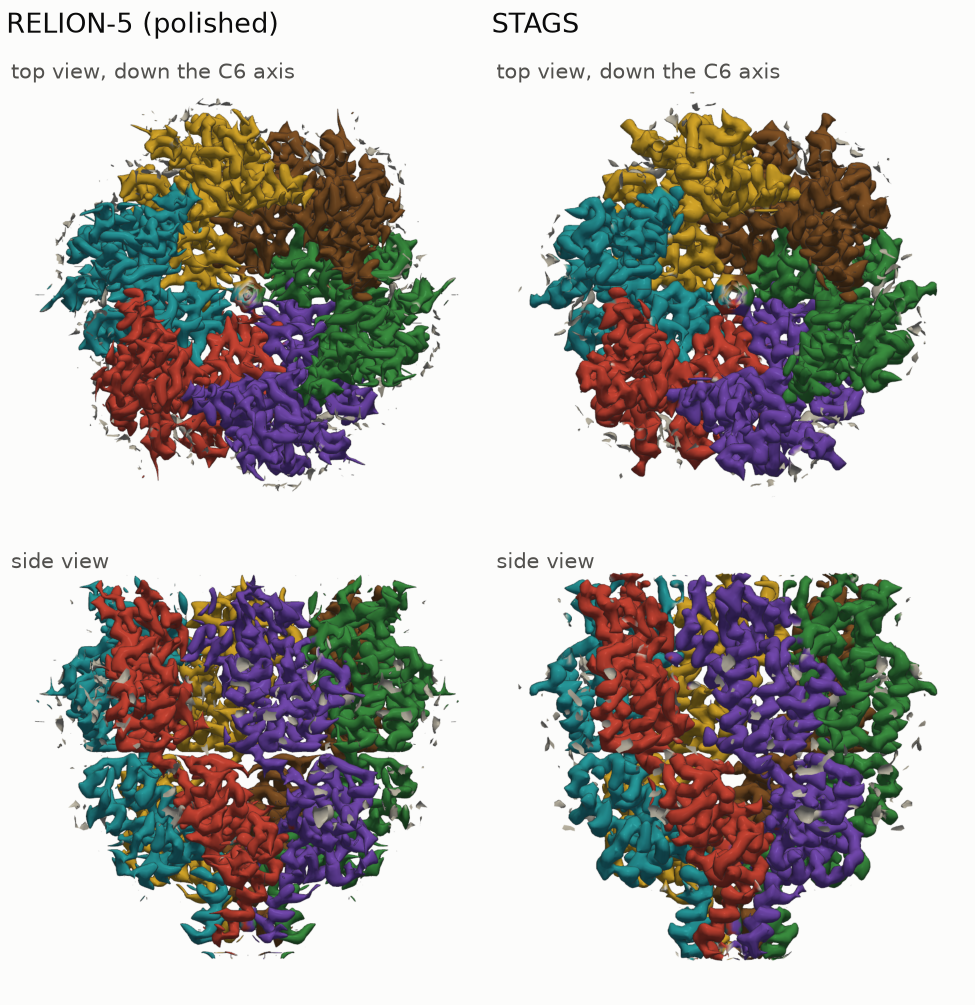
\includegraphics[width=\linewidth]{fig/abc_views.png}
\caption{\textbf{The two maps rendered identically.}
Top and side views of the central hexamer, RELION-5 polished map (left) and STAGS (right), colored by the nearest 5L93 subunit and zoned 4\,\AA\ around chains A1--A6.
Both maps: average of the two normalized half maps, the same B-factor ($-82.70$\,\AA$^2$, from RELION's post-processing job), the same raised-cosine low-pass from 3.5 to 3.1\,\AA, z-scored inside RELION's mask and thresholded to enclose the same volume, 101,942\,\AA$^3$ inside the mask (0.35$\times$ the molecular volume of the 5L93 residues inside the mask, the fraction at which RELION's map matches the silhouettes of its published Fig.~6C~\cite{burt2024relion5}); identical Taubin smoothing and cameras.}
\label{fig:views}
\end{figure}

\begin{figure*}[t]
\centering
% src: fig/abc_slices.png by scripts/paper_figures_abc.py; docs/paper/fig_abc_slices.csv; docs/paper/fig_abc_provenance.json (slices: sections z,y,x = 106, 96, 95; gray range z = -2.18 ... 4.47)
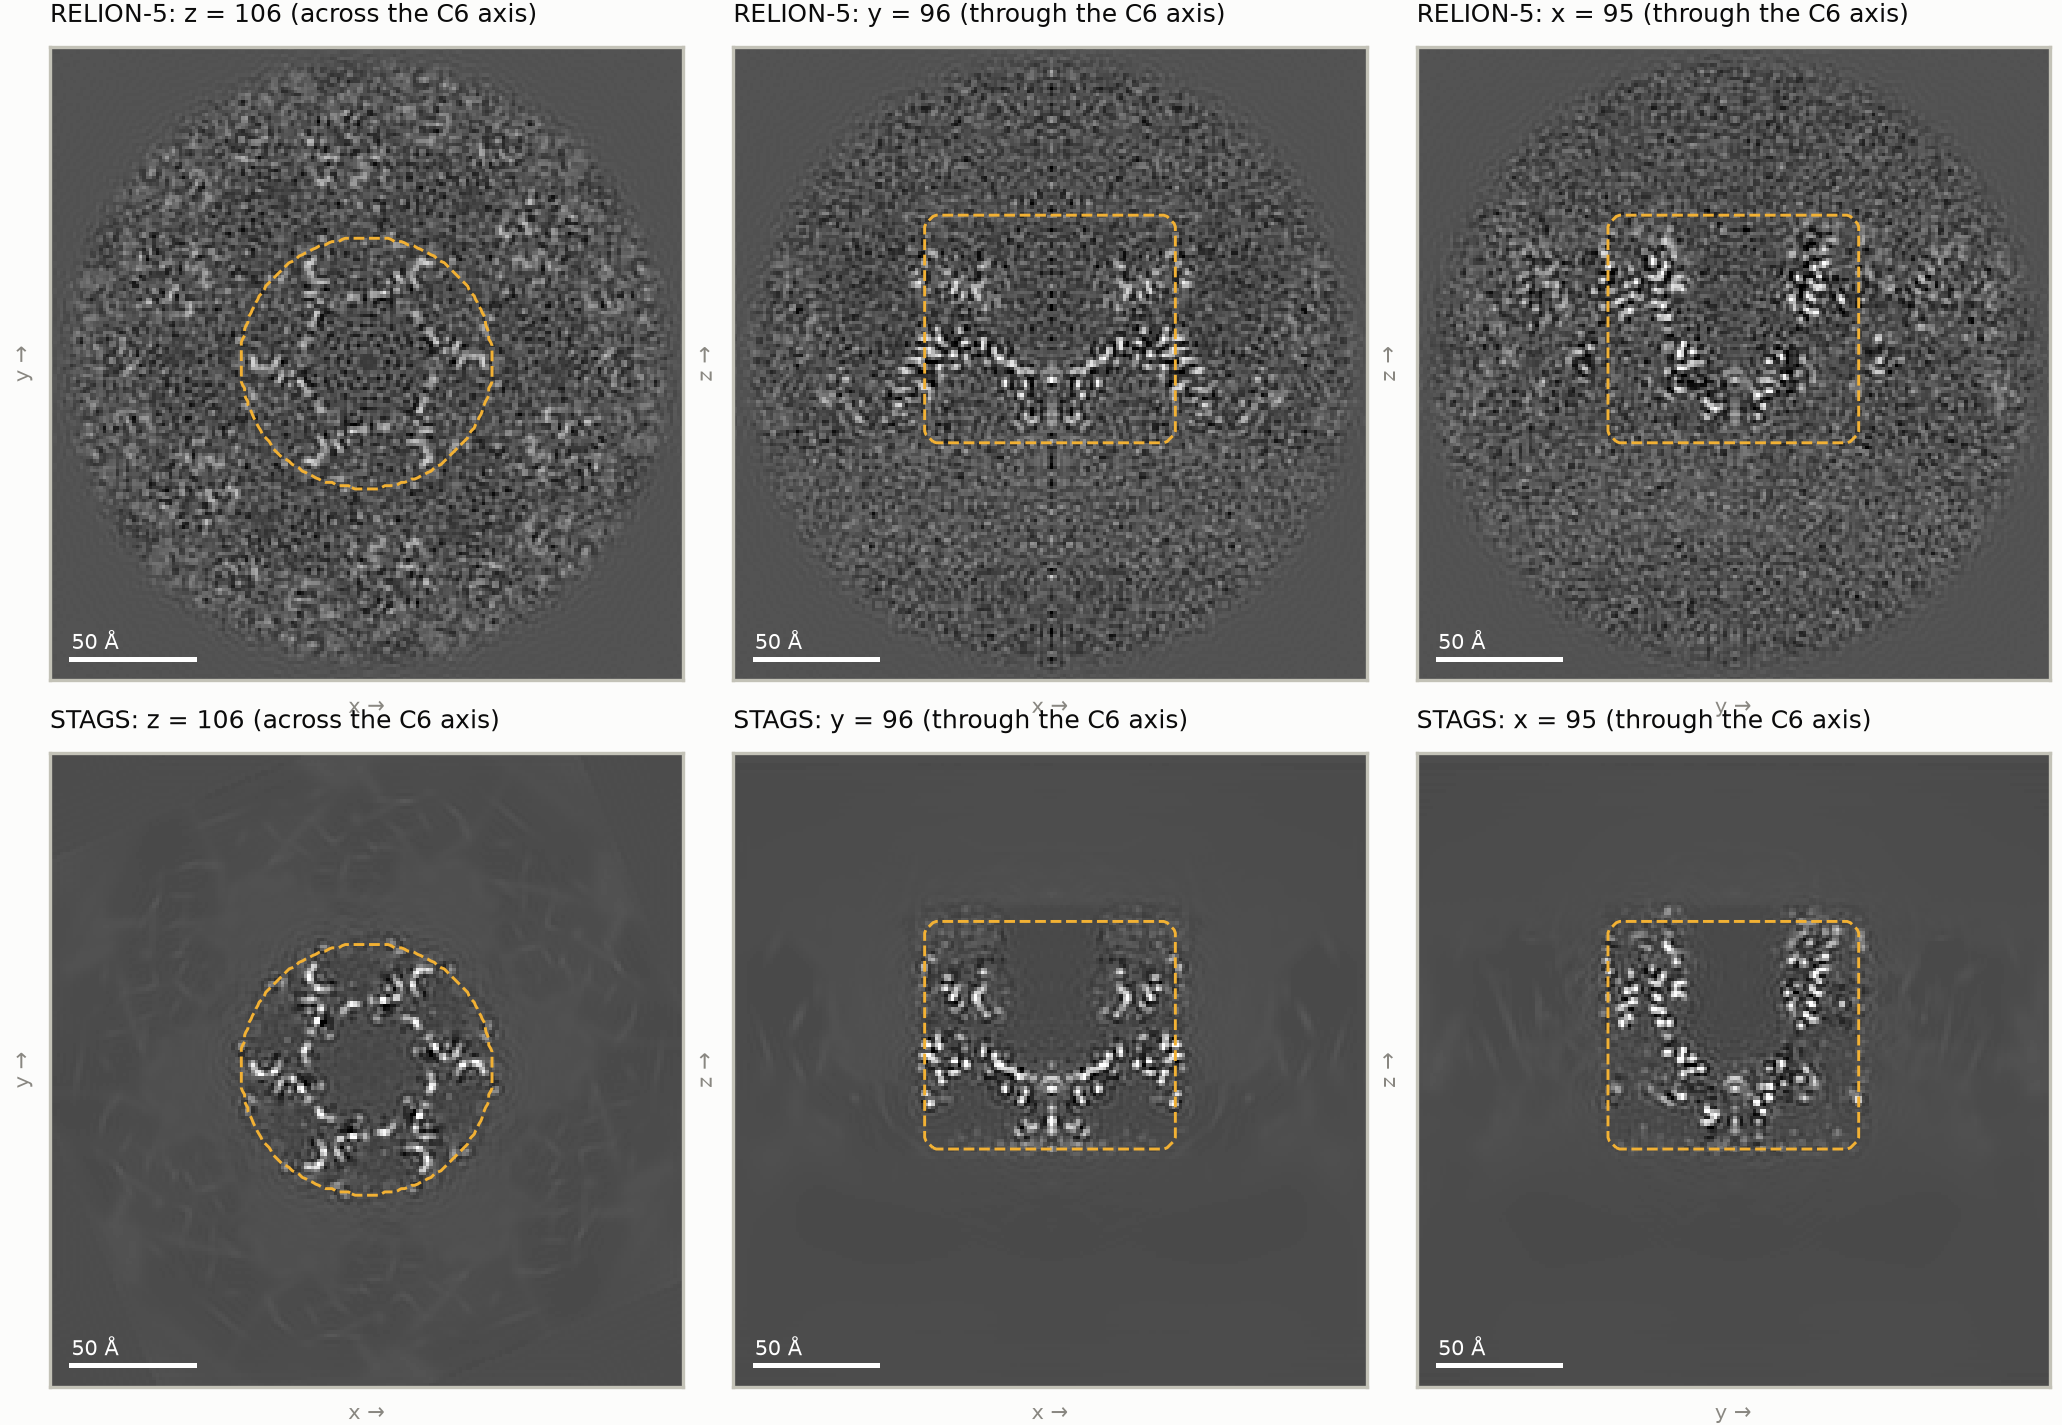
\includegraphics[width=\textwidth]{fig/abc_slices.png}
\caption{\textbf{Central sections, unmasked.}
Top, RELION-5 polished map; bottom, STAGS; one section across and two through the C6 axis.
Same filtering as \cref{fig:views}, z-scored inside RELION's mask (dashed outline), one common gray scale (0.5--99.5\,\% of both maps inside the mask).
Lattice neighbors outside the mask appear only in RELION's map.}
% src: docs/final-campaign-nov13.md (Visual comparison: "STAGS has no density outside its own mask")
\label{fig:slices}
\end{figure*}


\section{Pose-correction ablation}
\label{sec:suppl:ablation}

\begin{table}[t]
\centering
\resizebox{\linewidth}{!}{%
\begin{tabular}{@{}lccccc@{}}
\toprule
& cross-FSC 0.143 (\AA) & gain vs.\ control (\AA) & mean FSC 3.6--3.28\,\AA & 5L93 & gate \\
Arm (one cycle from frozen run E) & half 1 / half 2 & half 1 / half 2 & half 1 / half 2 & FSC 0.5 (\AA) & decision \\
\midrule
% rows generated by scripts/paper_figures_cvpr.py (tab_ablation)
\csname @@input\endcsname fig/tab_ablation_rows.tex
\bottomrule
\end{tabular}}
\caption{\textbf{Pose-correction ablation.}
Each arm continues the frozen final state of run~E for one cycle (local pose search, polishing, map refit) and is scored like \cref{tab:benchmark}.
Predeclared gate: a gain $>0.03$\,\AA\ on each half against both the control and the frozen state, with no worse 5L93 crossing.
No arm passed; a+b+c failed on half~2 ($^*$) and was adopted for the fresh run only after these results, on the band means (\cref{sec:results:ablation}).}
\label{tab:ablation}
\end{table}


\Cref{tab:ablation} tests three pose corrections, each in a matched one-cycle continuation from the frozen final state of run~E: (a)~exact Fourier-phase scoring of the final translation refinement, replacing bilinear interpolation, which drifts by 0.63\,\AA\ on known-answer fixtures where exact scoring drifts by 0.0002\,\AA; (b)~a masked Gaussian reference for the local pose search, with matching subtraction outside the mask; (c)~separate per-particle static translations and shared motion in polishing.
% src: docs/final-campaign-nov13.md (Step 1 recovery: 0.632614/0.625859 vs 0.000217/0.000210 A); runs/engine/posefix_20261113/recovery/report.json
The predeclared gate required a gain above 0.03\,\AA\ on each half, against both the continuation control and the frozen state, with no worse atomic agreement.
% src: engine_rules.json steps.posefix_20261113; docs/final-campaign-nov13.md (Frozen-E pose correction)
Alone, each change gains at most 0.021\,\AA; together they gain 0.082\,\AA\ on half~1 but only 0.015\,\AA\ on half~2, so the combination failed the gate.
% src: runs/engine/posefix_20261113/{a,b,c,abc}/result.json
Exact scoring inside the rotation-candidate ranking, evaluating every candidate, did not improve on the combination (0.064/0.013\,\AA) and was not adopted.
% src: runs/engine/pose_rank_exact_20261113/abc_exactrank/result.json; decision.json (blind_authorized=false)
We adopted the combination for the fresh run \emph{after} seeing these results: its mean FSC over 3.6--3.28\,\AA\ rose on both halves (+0.016/+0.017), its curves exceed the control's at every shell of that band, and its atomic agreement improved.
% src: docs/final-campaign-nov13.md (Explicit post-result adoption: +0.016170/+0.017196); runs/engine/pose_rank_exact_20261113/curve_diagnosis.json
The failed gate is not reclassified, and the selection after the result is part of why the benchmark is a development result rather than independent validation.

\section{Fixed-pose particle efficiency: details}
\label{sec:suppl:efficiency}

\paragraph{Withheld-tomogram study.}
The three splits withhold TS\_54, TS\_03 and TS\_45; the 250 training particles are drawn from the other four tomograms and 200 particles of the withheld tomogram are used only for image prediction.
% src: runs/native_limited250_20261103/selection.json (train TS_01/03/43/45; 250 train; 200 held out); docs/stags-limited-particle-study-matrix.md
The Gaussian map (48,000 Gaussians, 2,667 updates of 6 particles) is fitted to RELION's extracted particle images at 1.5$\times$ binning, with density outside the mask subtracted using a voxel map of the same 250 particles.
% src: engine_rules.json steps.A3_break_fixed_point.snr_gate.what; runs/step2_parity_20261103/score_primary/results.json (endpoint.recipe_differences)
It passes the predeclared margin of +0.01 FSC in every split, and its 5L93 crossing is slightly finer (7.08, 7.03, 7.05\,\AA\ against 7.23, 7.05, 7.16\,\AA).
% src: docs/results-limited250-three-study-20261103.md
The study's predeclared Gaussian arms (ray and wave models fitted to raw images at native sampling) failed against the voxel baseline (0.243 and 0.248 against 0.509); the reported recipe is an earlier one, substituted after that failure and scored under the same frozen gates.
% src: docs/results-limited250-primary-20261103.md
RELION-5 with 500 particles is better in all three splits (0.620, 0.601, 0.582), so the gain is not a halving of the particle count.
Image prediction on the withheld tomogram favors the Gaussian map (normalized squared error 0.99998 against 1.00074 in the first split), but an untrained Gaussian initialization already reaches most of that difference, and all methods explain almost none of the held-out signal.
% src: runs/native_limited250_20261103/native500_score/results.json (loss_over_observed_power); docs/results-limited250-primary-20261103.md (zero-update 0.99999)
All maps are scored against RELION's half-2 map, refined with the same poses, so the comparison is conditional on them.

\paragraph{Map-only control.}
The control fits the image-fit recipe's Gaussian initialization and schedule to the 250-particle voxel map.
% src: runs/native_limited250_20261103/control_v4_rules.json
It ran once, in the first split, without an adequacy gate, and scores 0.508 against 0.509 for the voxel map and 0.570 for the image-fitted Gaussians; its 5L93 crossing is much coarser (15.6\,\AA).
% src: runs/native_limited250_20261103/control_v4_outcome.json; map_only_control_v4/score/results.json
Three earlier versions failed the study's predeclared adequacy requirement, a relative $L_2$ error below 0.10 against the voxel map (1.15, 0.88 and 0.96); the 250-particle map is noise-dominated beyond 8\,\AA\ (97\,\% of its power), so a representation that does not copy its noise cannot meet that requirement.
% src: runs/native_limited250_20261103/map_only_control/decision.json (1.1506); controls_v2_outcome.json (0.883); control_v3_outcome.json (0.956; power beyond 8 A 0.973)
The control therefore supports, but does not prove, attributing the gain to the image-level fit.

\paragraph{Five-draw study.}
Five disjoint draws of 250 half-1 particles (nested in 500) with 200 further particles reserved compare raw-image Gaussian fits with a matched ridge-regularized voxel solver and with Gaussians fitted to each voxel-250 map.
% src: docs/results-stags-next-evaluation.md (particle-efficiency study)
Over 6.5--5.6\,\AA\ the Gaussian map exceeds the voxel-250 map by 0.175 (95\,\% CI [0.146, 0.203]) and the map-only fit by 0.137 [0.105, 0.169], and at 6.5\,\AA\ the voxel-500 map by 0.095 [0.064, 0.125].
% src: runs/particle_efficiency_20261102/results.json (comparisons A250, AG250, A500)
The map-only fits approximate their targets with a relative $L_2$ error of 0.98, so they are not an adequate smoothing control, and the Gaussian map predicts the reserved particles' images worse than the voxel-500 map in all five draws.
% src: runs/particle_efficiency_20261102/draw*/AG250/results.json (relative_map_l2 0.9789-0.9802); docs/results-stags-next-evaluation.md (reserved-particle prediction)

\section{Pipeline stage decisions}
\label{sec:suppl:part2}

Before the pose corrections of \cref{sec:suppl:ablation}, each stage of the pipeline was revisited with a predeclared keep rule on a short proxy: a cold map fit from the stage's output, or one refinement cycle, scored as in \cref{sec:results:setup}.
\Cref{tab:part2} lists every tested change.
The proxies have a noise floor of about $\pm$0.02--0.03\,\AA, visible as gains of opposite sign on the two halves.
% src: docs/final-campaign-nov13.md (Part 2, stage2_fit note: proxy noise floor)
Two decisions were revised after their results and are marked as such: the coarse-to-fine schedule stops at 5.5\,\AA\ (saving 58\,min) although the rule rejected it on half~2 by 0.032\,\AA, after a later fresh run with that stop gave a better proxy (3.881/3.886\,\AA) and the spread between runs was seen to be about 0.1\,\AA; and the revised optics scan was kept although its one-cycle proxy was within noise, because the previous scan failed a known-answer test (median defocus offset 225\,\AA\ recovered for a true 400\,\AA, against 397\,\AA\ for the revised scan) and the revised scan roughly halves the defocus deviation from RELION's refined values (median 118/141\,\AA\ against 221/217\,\AA).
% src: docs/final-campaign-nov13.md (stage1_ladder caveat_recorded_after and decision_revised_after; stage4_scan known_answer_h1, relion_diagnostic, DEVIATION recorded after the result)

\begin{table}[h]
\centering
\resizebox{\linewidth}{!}{%
\begin{tabular}{@{}llccl@{}}
\toprule
Stage & Change & Proxy (\AA) & Reference (\AA) & Decision \\
& & half 1 / half 2 & half 1 / half 2 & \\
\midrule
% src: docs/final-campaign-nov13.md (Part 2: stage1_ladder)
Schedule & stop at 5.5\,\AA\ ($-58$\,min) & 3.907 / 4.041 & 3.924 / 4.009 & reject; kept after result \\
% src: docs/final-campaign-nov13.md (Part 2: stage2_fit)
Map fit & fit band ends at 3.0\,\AA & 3.948 / 3.993 & 3.924 / 4.009 & reject \\
% src: docs/final-campaign-nov13.md (Part 2: stage3_p2 outcome)
Pose search & posterior mean, 4 rounds, FSC-weighted reference & 3.903 / 3.821 & 3.580 / 3.639 & reject \\
& top-8 mean, 3 rounds & 3.608 / 3.659 & 3.580 / 3.639 & reject \\
& posterior mean, 3 rounds, no weighting & 3.642 / 3.655 & 3.580 / 3.639 & reject \\
% src: docs/final-campaign-nov13.md (Part 2: stage4_scan proxy)
Optics scan & 384\,px raw, priors, every cycle ($+7.4$\,min) & 3.600 / 3.582 & 3.595 / 3.572 & reject; kept after result \\
% src: docs/final-campaign-nov13.md (Part 2: stage5_p1)
Polishing & damped motion model, capped steps ($-8$\,min) & 3.566 / 3.430 & 3.579 / 3.455 & keep \\
\bottomrule
\end{tabular}}
\caption{\textbf{Stage-by-stage decisions} (cross-FSC 0.143 crossings of the proxy and of its reference, lower is better). ``Kept after result'' marks decisions revised after the proxy was observed; the reasons are given in the text.}
\label{tab:part2}
\end{table}
